\section{Neural Architecture}

The implementation of ECC's principles through bioenergetic mechanisms depends critically on the brain's underlying structural organization. Neural architecture provides the physical substrate that enables both efficient energy distribution and the maintenance of coherent conscious states. This organization reflects evolutionary optimization for both information processing and energy management, creating what can be described as structured efficiency in biological systems \cite{Hilgetag2020}.

The layered organization of the cortex serves as an ideal physical structure for implementing ECC's principles of energetic coherence and information integration \cite{Douglas2004}. The distinct laminar organization, with its carefully regulated ratios of excitatory and inhibitory neurons, establishes coherence domains - regions where energy flows can be locally stabilized while maintaining dynamic coupling with adjacent areas \cite{Harris2015}.

Cortical columns emerge as particularly significant architectural features, forming natural units for maintaining local energetic coherence \cite{Mountcastle1997}. These columns, extending vertically through cortical layers, create coherence channels that enable several crucial functions. They facilitate efficient vertical integration of information across cortical layers while providing contained units for local stabilization of energy dynamics. The balanced ratios of excitation and inhibition within these columns help maintain low-entropy states, while their structure creates natural boundaries for the sheaf-theoretic sections described in the mathematical formalism.

The horizontal organization of cortical tissue proves equally important, with its dense network of lateral connections forming coherence coupling zones \cite{DeFelipe2011}. These zones enable the propagation of coherent states between adjacent columns and support the distribution of energy loads across the cortical sheet. This horizontal architecture implements the \textit{gluing} operations described in the sheaf-theoretic framework while enabling the creation of larger-scale coherent fields from local stable states.

White matter architecture plays an essential role beyond mere connectivity \cite{Sporns2011}. Long-range fiber tracts serve as coherence bridges that help maintain global stability of conscious states. The precise topology of these connections appears to reflect evolutionary optimization for both minimal wiring length, reducing energy costs, and maximal maintenance of coherent fields across distributed regions. This architectural efficiency directly supports ECC's emphasis on low-entropy conscious states emerging from coherent energy dynamics.

Perhaps most crucial is the neuropil itself - the dense network of neural processes, glial cells, and extracellular matrix that fills the spaces between neuronal cell bodies \cite{Kasthuri2015}. This intricate mesh, supported by dendritic processes and their spines, creates the physical substrate necessary for maintaining coherent energy states and enabling state sharing across regions. The neuropil's architecture proves particularly well-suited for supporting brain waves, which ECC views as essential mechanisms for maintaining coherent states. Its dense connectivity and precise spatial organization allows for efficient propagation of oscillatory activity, local synchronization of neural populations, and the creation of standing waves that help stabilize conscious states.

\begin{figure}[h]
    \centering
    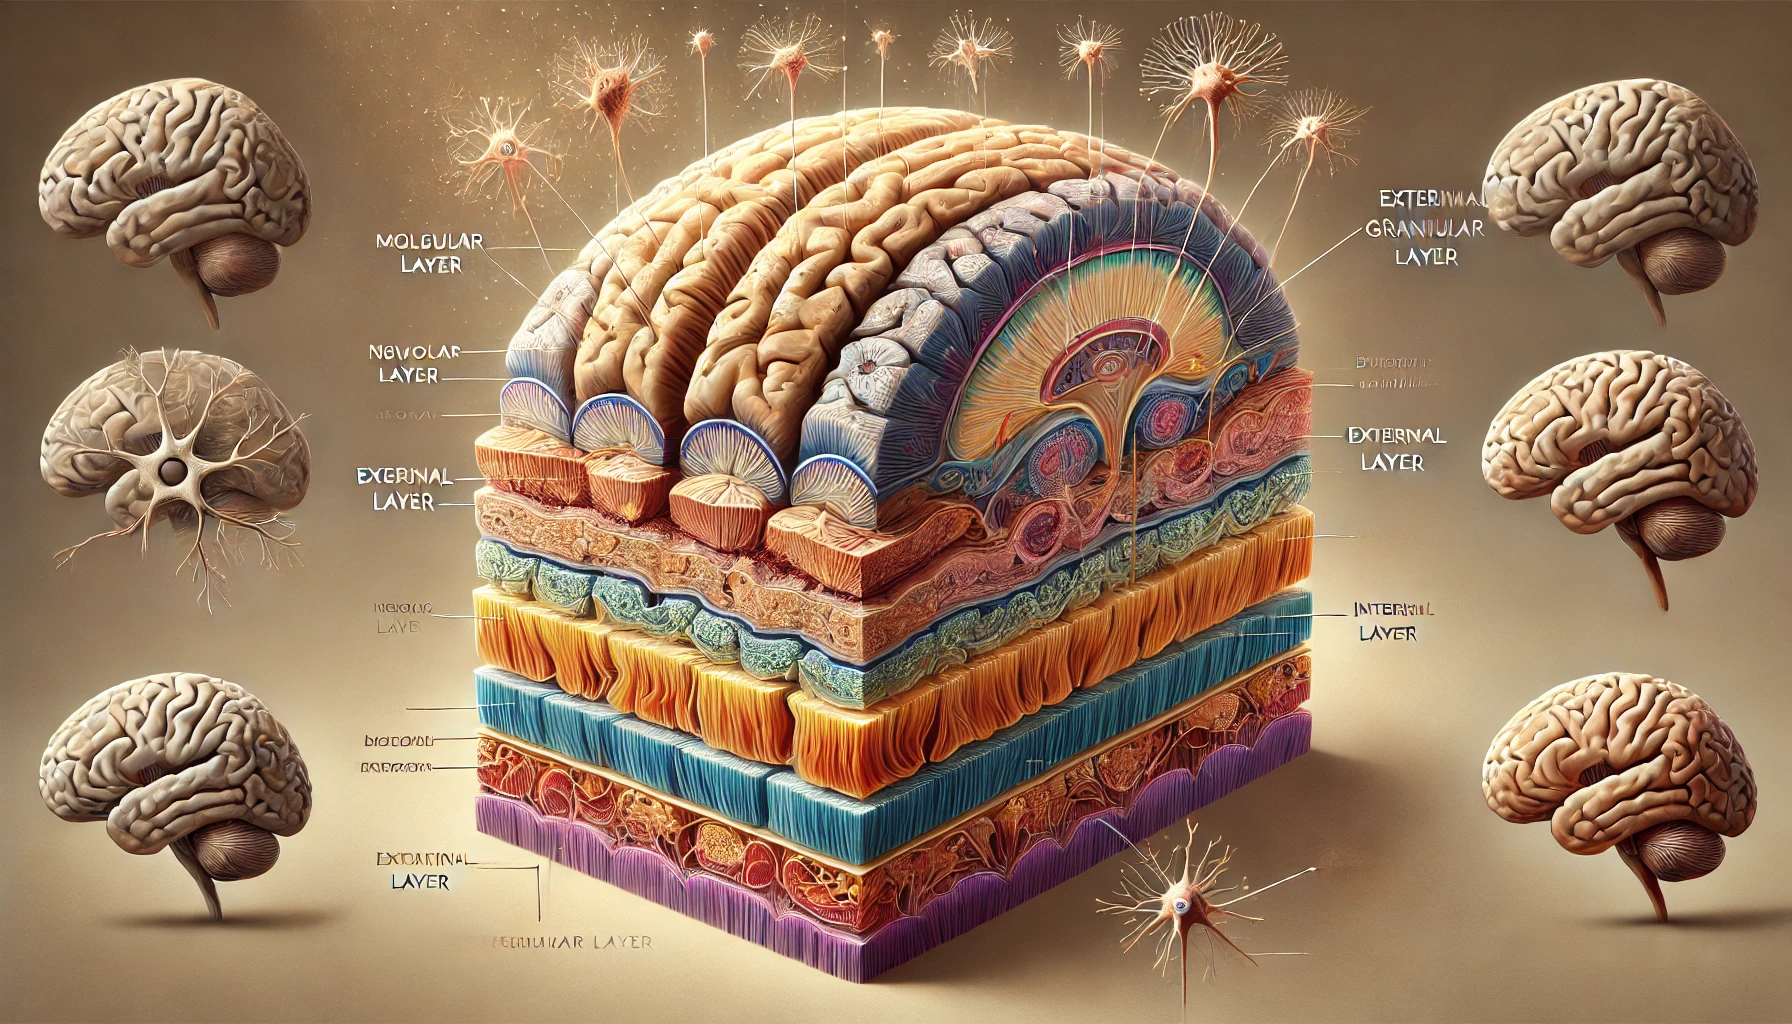
\includegraphics[width=0.8\textwidth]{cortical_layers.png}

    \caption{Cortical layers}
\end{figure}

The neuropil's dense connectivity serves multiple critical functions in maintaining conscious states \cite{Kasthuri2015}. Through its precise spatial organization, it enables coordinated interactions between neurons and glia while providing structured pathways for field-like effects to propagate. The arrangement of cellular processes creates an intricate three-dimensional matrix that supports both local processing and global integration of neural activity.

Astrocytic processes within the neuropil form an essential component of this architecture \cite{Peters1984}. Their elaborate branching patterns and strategic positioning allow them to monitor and modulate synaptic activity while maintaining ion homeostasis across substantial volumes of neural tissue. This spatial organization enables astrocytes to coordinate energy distribution and maintain coherent states across multiple spatial scales.

The extracellular matrix embedded within the neuropil provides another crucial architectural element \cite{Braitenberg1998}. Its molecular scaffolding helps stabilize synaptic connections while influencing the diffusion of neurotransmitters and ions. The precise composition and organization of the matrix varies across brain regions, creating specialized microenvironments that support different aspects of neural processing and energy management.

Dendritic architecture within the neuropil deserves particular attention \cite{Rockland2020}. The intricate branching patterns of dendrites create overlapping fields of integration that allow neurons to sample inputs from diverse sources while maintaining specific computational properties. This architectural feature enables sophisticated information processing while supporting the establishment of coherent energy states across neural populations.

The spatial arrangement of synaptic connections within the neuropil reflects both specific computational requirements and energy efficiency constraints \cite{Markram2015}. Synapses cluster in patterns that minimize wiring length while maximizing information transfer, creating local processing units that can maintain stable energy states while remaining dynamically responsive to changing inputs. This organization supports the emergence of coherent activity patterns while enabling flexible reconfiguration based on computational demands.

Gap junctions between cells provide another essential architectural feature within the neuropil \cite{Zeng2017}. These direct cellular connections create alternative pathways for signal propagation and state sharing, enabling rapid synchronization of cellular assemblies without requiring synaptic transmission. The distribution and regulation of gap junctions helps establish domains of coordinated activity that can maintain coherent states across multiple spatial scales.

The integration of these various architectural elements - astrocytic processes, extracellular matrix, dendritic fields, synaptic clusters, and gap junctions - creates a physical substrate capable of supporting the sophisticated energy dynamics required for conscious processing \cite{Bassett2017}. This multi-scale organization enables both local specialization and global integration while maintaining the energetic efficiency necessary for sustained conscious activity.

Through this architectural organization, the brain achieves a remarkable balance between stability and flexibility \cite{Buzsaki2006}. The structured pathways for energy flow and information processing allow for the maintenance of coherent states while enabling dynamic responses to changing conditions. This sophisticated architecture, refined through evolution, provides the physical foundation necessary for consciousness to emerge from organized energy flows within neural tissue.

The architectural organization of neural tissue culminates in a system that supports multiple modes of information transmission and energy propagation \cite{VanEssen2018}. Beyond classical synaptic transmission, the neuropil's structure enables ephaptic coupling, volume transmission, and field effects that contribute to conscious processing. These various mechanisms operate simultaneously across different spatial and temporal scales, creating a rich landscape of possible interactions that support coherent conscious states.

The evolutionary refinement of this architecture reflects a delicate balance between competing demands \cite{Hilgetag2020}. The need for efficient information processing must be weighed against energy constraints, while requirements for stability must accommodate the need for plasticity and adaptation. The resulting structure represents a sophisticated solution to these competing pressures, enabling conscious processing through carefully organized patterns of energy flow.

Perhaps most remarkably, this neural architecture creates conditions for emergent properties that transcend the capabilities of individual components \cite{vonBartheld2016}. Through its precise organization across multiple scales, from molecular arrangements to global connectivity patterns, the brain's structure enables the emergence of conscious experience from coherent energy dynamics. This emergence depends not just on the properties of individual elements but on their precise spatial arrangement and coordinated interaction.

Understanding neural architecture through the lens of ECC provides crucial insights into both the possibilities and constraints of conscious processing. The physical structure of neural tissue determines what patterns of energetic coherence can be maintained, what forms of information processing are possible, and what limitations must be respected. This architectural foundation proves essential for any complete theory of consciousness.